\documentclass[12pt]{standalone}
\usepackage{tikz}
\usepackage{verbatim}
\usepackage{microtype}
\usepackage{graphicx}
\usepackage{subfigure}
\usepackage{booktabs} % for professional tables
\begin{comment}
a
\end{comment}
\usepackage{pgfplots}
\pgfplotsset{compat=1.7}
\usepackage{tikz}
\usetikzlibrary{positioning,calc}
\usetikzlibrary{matrix}

\usepackage{setspace}

\begin{document}
\pagestyle{empty}


%%%%%%%%%%%%%%%%%%
% Figure from: Lanctot, Marc, Vinicius Zambaldi, Audrunas Gruslys, Angeliki Lazaridou, Karl Tuyls, Julien Pérolat, David Silver, and Thore Graepel. "A unified game-theoretic approach to multiagent reinforcement learning." In Advances in Neural Information Processing Systems, pp. 4190-4203. 2017.
%%%%%%%%%%%%%%%%%%%

% \begin{figure}
% \centering
% \begin{minipage}{0.45\textwidth}
% \hspace{0pt}
% \centering
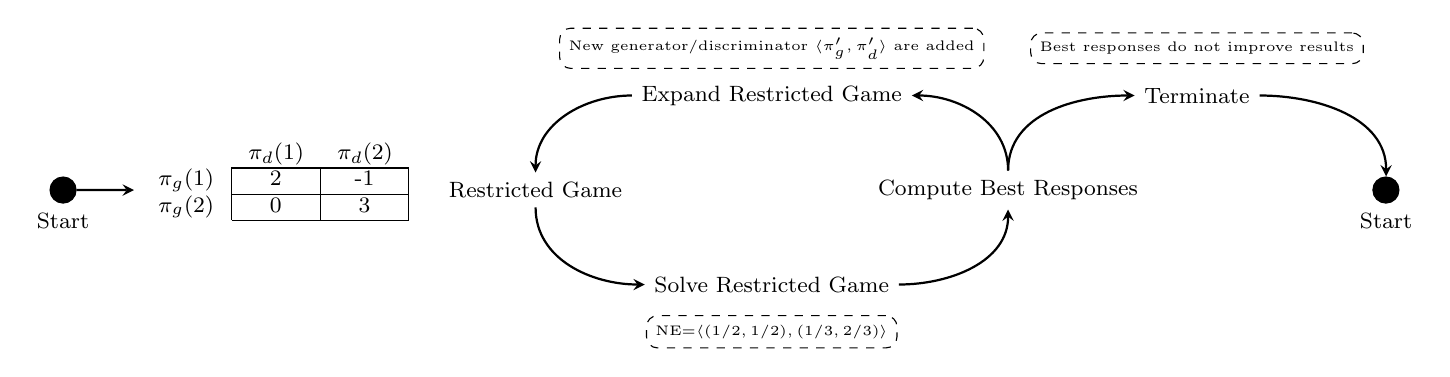
\begin{tikzpicture}[scale=1.2]
\path (-2, 2) node[draw, fill=black, shape=circle, label=below:{\footnotesize{Start}}] (start) {};

\path (3, 2) node (res_game) {\footnotesize{Restricted Game}};

\path (5.5, 1) node (solve_res_game) {\footnotesize{Solve Restricted Game}};
\path (5.5, 0.5) node[draw, dashed, rounded corners] (ne_strategy) {\tiny{NE=$\langle(1/2, 1/2),(1/3, 2/3)\rangle$}};

\path (8, 2) node (com_best_response) {\footnotesize{Compute Best Responses}};

\path (5.5, 3) node (expand_res_game) {\footnotesize{Expand Restricted Game}};
\path (5.5, 3.5) node[draw, dashed, rounded corners] (gen_dis_add) {\tiny{New generator/discriminator $\langle\pi'_{g}, \pi'_{d}\rangle$ are added}};

\path (10, 3) node (terminate) {\footnotesize{Terminate}};
\path (10, 3.5) node[draw, dashed, rounded corners] (best_improve) {\tiny{Best responses do not improve results}};


\path (12, 2) node[draw, fill=black, shape=circle, label=below:{\footnotesize{Start}}] (end) {};

\draw[thick, -stealth] (res_game.south) to[out=-90, in=180] (solve_res_game.west);
\draw[thick, -stealth] (solve_res_game.east) to[out=0, in=-90] (com_best_response.south);
\draw[thick, -stealth] (com_best_response.north) to[out=90, in=0] (expand_res_game.east);
\draw[thick, -stealth] (com_best_response.north) to[out=90, in=180] (terminate.west);
\draw[thick, -stealth] (terminate.east) to[out=0, in=90] (end.north);
\draw[thick, -stealth] (expand_res_game.west) to[out=180, in=90] (res_game.north);

% draw payoff matrix
% \path (0, 2) node (aO) {};
% \path (aO++(0.25, 0.25)) node (a11) {1};
% \path (0.75, 2.25) node (a11) {1};
% \path (0.25, 1.75) node (a11) {1};
% \path (0.75, 1.75) node (a11) {1};

% \path (-0.1, 2.25) node (a11) {$\pi_{g}(1)$};
% \halign{\it#\tabskip=1em & \hfil#\hfil & \hfil\$#\cr
% China & Apple & 1.0\cr
% France & Banana & 0.574\cr}
% \matrix (magic) [matrix of nodes]
% {
%  & \footnotesize{$\pi_{d}(1)$} & \footnotesize{$\pi_{d}(2)$} \\\hline
% \footnotesize{$\pi_{g}(1)$} & \footnotesize{2} & \footnotesize{-1} \\\hline
% \footnotesize{$\pi_{g}(2)$} & \footnotesize{0} & \footnotesize{3} \\
% };

\path (0.25, 2.1) node (payoff) {\footnotesize{
% \begin{spacing}{1.19}
\begin{tabular}{c|c|c|}
% \arraystretch{1.5}
% \cline{2-3}
\multicolumn{1}{c}{}& \multicolumn{1}{c}{$\pi_{d}(1)$} & \multicolumn{1}{c}{$\pi_{d}(2)$}\\\cline{2-3}
$\pi_{g}(1)$ & 2 & -1 \\\cline{2-3}
$\pi_{g}(2)$ & 0 & 3 \\\cline{2-3}
\end{tabular}
% \end{spacing}
}
};

\draw[-stealth, thick] (start) -- (-1.25, 2);
\end{tikzpicture}


\end{document} 